\section{Design}\label{sec:design}

In this section we describe the design of \softtcp, with the following design
goals:

\begin{compactitem}[\labelitemi]
\item \textbf{Efficiency:} Data center network bandwidth growth
  continues to outpace processor performance. \softtcp must deliver
  CPU efficient packet processing, especially for latency-sensitive
  small packet communication that is the common case behavior for data
  center applications and services.

\item \textbf{Connection scalability:} As applications and services
  scale up to larger numbers of servers inside the data center,
  incast, where a single server handles a large number of connections,
  continues to grow. \softtcp must support this increasing number of
  connections.

\item \textbf{Performance predictability:} Another consequence of this
  scale is that predictable performance is becoming as important as
  high common case performance for many applications.  In large-scale
  systems, individual user requests can access thousands of backend
  servers~\cite{jalaparti:taillatency,nishtala:memcache_facebook}
  causing one-in-a-thousand request performance to determine common
  case performance.

\item \textbf{Policy compliance:} Applications from different tenants
  must be prevented from intercepting and interfering with network
  communication from other tenants. Thus, \softtcp must be able to
  enforce policies such as bandwidth limits, memory isolation,
  firewalls, and congestion control.

\item \textbf{Workload proportionality:} \softtcp should not use more
  CPUs than necessary to provide the required throughput for the
  application workloads running on the server. This requires \softtcp
  to scale its CPU usage up and down, depending on demand.

  %\item \textbf{Protocol Flexibility:}
  %  Data centers are a fast moving environment.
  %  Network infrastructure is evolving and data center network protocols are an
  %  active area of research.
  %  New applications are also constantly being rolled out and existing
  %  applications are evolving, leading to changes in application protocols,
  %  architecture, and performance characteristics.
  %  Packet processing must be flexible in adapting to new protocols, network
  %  infrastructure, and application requirements.

  %\item \textbf{Cost Efficiency:}
  %  Finally, any architecture for accelerating packet processing has to be
  %  economical.
  %  The total cost of ownership factors in hardware cost, available processor
  %  capacity for applications, and energy.
  %  For hardware cost, I use chip area as a proxy.
  %  Costs for hardware extensions, for example, must be justified by reduced
  %  processor time for software processing or reduced energy consumption.
\end{compactitem}

\begin{figure}
  \centering
  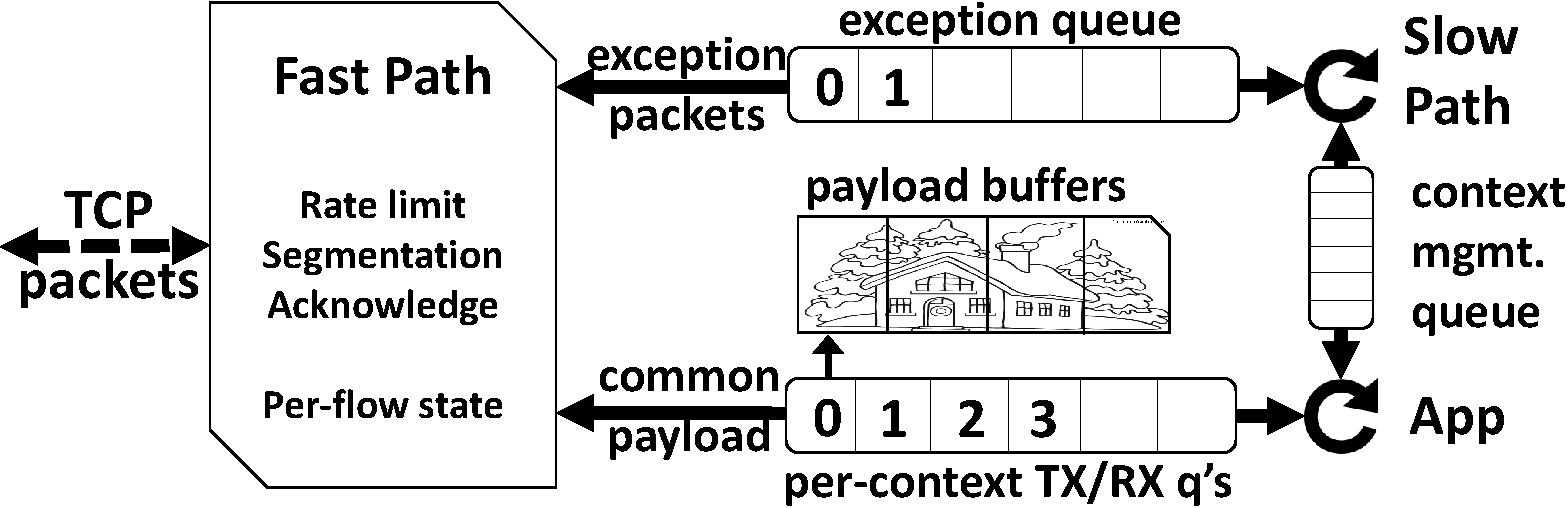
\includegraphics[width=\columnwidth]{rmttcp_design-crop}
  \caption{\softtcp Design. Per-flow state is in the fast path, the exception
    queue is shared by the fast path and the slow path, and everything else
    is in user memory.}
  \label{fig:softtcp}
\end{figure}

Figure~\ref{fig:softtcp} shows an overview of \softtcp. \softtcp has
three components: Fast path, slow path, and untrusted per-application
user-space stack. All components are connected via a series of shared
memory queues, optimized for cache-efficient message
passing~\cite{barrelfish}. The fast path is responsible for handling
common case packet exchanges. To do so, it deposits the payload of
incoming packets directly in user-space per-flow \emph{receive payload
  buffers}, notifying the user-space TCP stack of data arrival via a
\emph{receive context queue}. Outgoing payload is written by the
user-space TCP stack into per-flow \emph{transmit payload buffers},
notifying the fast path via a \emph{transmit context queue}. The fast
path fetches and encapsulates payload according to per-connection
\emph{rate limits} that are dynamically configured by the slow path.
% To encapsulate payload, the NIC maintains per-flow local
% and peer TCP sequence numbers.
User-level TCP stacks provide the standard POSIX API to applications.
Applications do not need to be modified but do need to be relinked.
For connection setup and teardown, each user-level stack interacts
with the slow path using \emph{slow path context queues}.

\subsection{Fast Path Functionality}

The fast path handles common-case exchange of packets on established
connections. It also must detect and respond to exceptions, such as
out-of-order arrivals and unknown connections, and enforce congestion
policy. It processes protocol headers, sends TCP acknowledgments, and
performs segmentation.

\paragraph{Common-case receive.} \softtcp assumes that packets are
commonly delivered in order by the network. This is true for data
center networks today due to connection-stable multi-path
routing~\cite{vl2,jupiter}. With in order packets, the fast path can
discard all network headers and directly insert the payload into a
user-level, per-flow, circular payload receive buffer. The fast path
can directly write received payload to user memory, notifying an
appropriate context queue by identifying the connection and number of
bytes received. When a payload buffer is full, the fast path simply
drops the packet. When a context queue is full, the fast path will
inform the user-level stack upon future packet arrivals if the queue
is available. User-level stacks are free to define and configure
contexts. We describe them in more detail in
Section~\ref{sec:app_design}.

Per-flow payload buffers simplify packet handling, flow control, and
improve isolation.  Calculating an accurate flow control window with
shared buffers requires iteration over all connections sharing the
buffer, imposing non-constant per-packet overhead.

\paragraph{Fast path generated ACKs.} After depositing the payload of
an in-order packet, the fast path automatically generates an
acknowledgement packet and transmits it to the sender to update its
TCP window. Handling TCP acknowledgements in \taas is important for
security. If user-space was given control over acknowledgements, as in
many kernel-bypass solutions, it can use it to defeat TCP congestion
control \cite{misbehaving_receivers_ccr_1999}.  The acknowledgements
also provide correct ECN feedback, and accurate TCP timestamps for RTT
estimation.

 % (and number of bytes sent and
% acknowledged on that connection as an optimization).
% To do so, the NIC parses the TCP
% header, looks up the flow state, and after validating the sequence
% number and packet header, writes the notification to the per-core
% receive queue indicated in the flow state.
 % An \emph{exception queue} is provided by the
% kernel to handle out-of-order, lost, and unrecognized packets, as well
% as to receive congestion information and control NIC state and rate
% limits.
% Congestion and acknowledgement information is
% directed to appropriate handling queues.

\paragraph{Common-case send.} User-level stacks send data on a flow by
appending it to a flow's circular transmit buffer. Per-flow send
buffers are required to alleviate head-of-line blocking under rate and
flow control. To inform the fast path, the stack issues a TX command
on a context queue and sets a doorbell.  The fast path fills a
flow-specific QM bucket with the new amount of data to
send. Asynchronously, the QM drains these buckets, depending on the
configured rate-limit and the receiver's TCP window, to enforce
congestion and flow control. When data can be sent, the fast path
fetches the appropriate amount from the transmit buffer, produces TCP
segments, prepends packet headers for the connection, and
transmits. % This realizes TCP segmentation independent of application
% transmit granularity.

\paragraph{ACK processing.} Any payload that has been sent remains in
the transmit buffer until acknowledged by the receiver. The fast path
parses incoming acknowledgements, updates per-flow sequence and window
state, frees transmit payload buffer space, and informs user-space of
reliably delivered packets by issuing a notification with the number
of transmitted bytes for the corresponding flow. This requires
constant time. The fast path also uses TCP timestamps to provide the
slow path with an accurate RTT estimate for congestion control and
timeouts.
% \antoine{not sure where this should go? We could also cite TIMELY,
% which argues for NIC timestamping to reduce noise in RTT estimation}.

\paragraph{Fast path state.} To enforce policy, the fast path requires
the per-flow state shown in Table~\ref{tab:nic_state}. The opaque
field is specified by and relayed to user-space to help it identify
the corresponding connection. Similarly, the doorbell register helps
the fast path identify what per-core receive and transmit queue to
use.  RX/TX buffer state is used for management of per-flow buffers in
user-space.  The slow path can access fast path state via shared
memory.  In all, we require 102 bytes of per-flow state. Current
commodity server CPUs supply about 2MB of L2/3 data cache per core
($\S$\ref{sec:impl}). This allows us to keep the state of more than
20,000 active flows per core in the fast path. Packets for any flows
that do not fit are directed to the slow path queue and processed in
the slow path. Integrating ideas to reduce fast path state (e.g.,
SENIC~\cite{senic}) is future work.

\paragraph{Exceptions.} The fast path detects out-of-order arrivals by
matching arrivals against expected sequence numbers in the per-flow
\verb+seq+ register. It drops them and generates an acknowledgement
specifying the next expected sequence number.  When processing
incoming acknowledgements the fast path counts duplicates and triggers
fast recovery after three duplicates, without slow path intervention,
by resetting the sender state as if those segments had not been
sent. The fast path also increments a per-flow retransmit counter to
inform the slow path to reduce the flow's rate limit.
% The kernel manages retransmission timeouts as described below.

As an optimization, the fast path tracks one interval of out-of-order
data in the receive buffer (starting at \verb+ooo_start+ and of length
\verb+ooo_len+).  The fast path accepts out-of-order segments of the
same interval if they fit in the receive buffer. In that case, the
fast path writes the payload to the corresponding position in the
receive buffer.  When an in-order segment fills the gap between
existing stream and interval, the fast path notifies the user-level
stack as if one big segment arrived, and resets its out-of-order
state.

Other exceptions, such as unidentified connections, corrupted packets,
and packets with unhandled flags, are filtered and sent to the
slow path for processing.

\subsection{Slow Path}

The slow path implements all policy decisions and management
mechanisms that have non-constant per packet overhead or are too
expensive or stateful to process in the fast path. This includes
congestion control policy, connection management, user-space TCP stack
registry, handling timeouts and other exceptional situations.

\paragraph{Congestion control.} \softtcp enforces congestion control
by configuring the fast path to limit each connection to a specific
rate.  The slow path updates flow rates periodically out-of-band,
based on congestion feedback collected by the fast path.  Based on
received ACKs, the fast path maintains for each flow: bytes
acknowledged with and without ECN marks, number of fast retransmits,
and current RTT estimate.  The fast path runs a control loop iteration
for each flow every control interval (configurable, by default every 2
RTTs).  It retrieves congestion feedback from the fast path, then runs
a congestion control algorithm to calculate a new flow rate, and
finally updates the flow rate in the fast path via shared memory.

This provides a generic framework to implement different congestion
control algorithms.  We implement DCTCP~\cite{dctcp} and
TIMELY~\cite{timely} (adapted for TCP by adding slow-start).  We adapt
DCTCP to operate on rates instead of windows by applying its control
law (rate-decrease proportional to fraction of ECN marked bytes) to
flow rates.  During slow start we double the rate every control
interval until there is an indication of congestion, and during
additive increase we add a configurable step size (10mbps by default)
to the current rate.  To prevent rates from growing arbitrarily in
absence of congestion, we ensure at the beginning of the control loop
that the rate is no more than 20\% higher than the flow's send rate.
Our rate-based DCTCP implementation is compatible with Linux peers.

%\paragraph{Explicit congestion control.} \softtcp implements
%DCTCP-style congestion control~\cite{dctcp} based on explicit
%congestion notification (ECN). DCTCP consists of two parts: reflecting
%ECN bits to the sender, and processing incoming congestion
%notifications.  We make three peer-compatible changes to DCTCP to
%allow for an efficient implementation in our design.  First, \softtcp
%does not use delayed acknowledgements but acknowledges every packet.
%Thus, the NIC reflects the ECN bit back to the sender when generating
%the acknowledgement instead of using a state machine to determine when
%to acknowledge. Second, to reduce bursts and to enforce fairness among
%multiple user-space TCP stacks, we use rate limits instead of a window
%based protocol. Third, instead of adjusting the rate each time the NIC
%receives a packet, \softtcp collects statistics on the fraction of
%packets of the flow that experienced congestion. The kernel
%periodically collects those statistics and updates the rate limits,
%via NIC configuration registers, according to the DCTCP control law.
%We show that these changes have limited impact on DCTCP effectiveness.
%Our goal is to be able to support a variety of congestion control
%protocols; it remains future work to understand how best to implement
%these with rate limits.

\paragraph{Stack management.} To associate new user-space TCP stacks
with \softtcp, the slow path has to be informed via a special system
call. If the request is granted, the slow path creates an initial pair
of context queues that the user-space stack uses to create connection
buffers, etc.
% and a new virtual NIC is mapped directly into the application address
% space using I/O virtualization~\cite{sriov}. 
% The virtual NIC provides and is mapped directly into the address space of the
% application. 
% This mechanism is identical to that in the Arrakis OS~\cite{peter:arrakis}.

\begin{table}
  \centering
  \small
  \begin{tabular}{lrl}
    \textbf{Register} & \textbf{Bits} & \textbf{Description} \\
    \hline
    \verb+opaque+ & 64 & Application-defined flow identifier \\
    \verb+doorbell+ & 16 & Associated TX doorbell \\
    \verb+bucket+ & 24 & Associated QM bucket ID \\
    \verb+rx|tx_start+ & 128 & RX/TX buffer start \\
    \verb+rx|tx_size+ & 64 & RX/TX buffer size \\
    \verb+rx|tx_head|tail+ & 128 & RX/TX buffer head/tail position \\
    \verb+tx_sent+ & 32 & Sent bytes from \verb+tx_head+ \\
    \verb+seq+ & 32 & Local TCP sequence number \\
    \verb+ack+ & 32 & Peer TCP sequence number \\
    \verb+window+ & 16 & Remote TCP receive window \\
    \verb+dupack_cnt+ & 4 & Duplicate ACK count \\
    \verb+local_port+ & 16 & Local port number \\
    \verb+peer_ip|port|mac+ & 96 & Peer 3-tuple (for segmentation) \\
    \verb+ooo_start|len+ & 64 & Out-of-order interval \\
    \verb+cnt_ackb|ecnb+ & 64 & ACK'd and ECN marked bytes \\
    \verb+cnt_frexmits+ & 8 & Fast re-transmits triggered count \\
    \verb+rtt_est+ & 32 & RTT estimate \\
  \end{tabular}
  \caption{Required per-flow fast path state (102 bytes total).}
  \label{tab:nic_state}
\end{table}

\paragraph{Connection management.} Connection management is
complex. It includes port allocation, negotiation of TCP options,
maintaining ARP tables, and IP routing. We thus handle it in the slow
path. User-level TCP stacks issue a \verb+new_flow+ command on the
slow path context queue to locally request new connections. If
granted, the slow path establishes the connection by executing the TCP
handshake in software and, if successful, installs the established
flow's state in the fast path and allocates a rate-limited QM
bucket. Remote requests are detected by the fast path and forwarded to
the slow path, which then completes the handshake.

Servers can listen on a port by issuing a \verb+listen+ command to the
slow path. The slow path informs user-space of incoming connections on
registered ports by posting a notification in the slow path context
queue. If user-space decides to accept the connection, it may issue
the \verb+accept+ command to the slow path (via the slow path context
queue), upon which the slow path establishes the flow. To tear down a
connection, user-space issues \verb+close+, upon which the slow path
executes the appropriate handshake and removes the flow state from the
fast path. Similarly, for remote teardowns, the slow path informs
user-space via a \verb+close+ command.

\paragraph{Retransmission timeouts.} We handle retransmission timeouts
in the slow path. When collecting congestion statistics for a flow
from the fast path, the kernel also checks for unacknowledged
data. % in its send buffer
% and the start sequence number of that data
If a flow has unacknowledged data with a constant sequence number for
multiple control intervals (2 by default) the slow path instructs the
fast path to start retransmitting by adding a command to the slow path
context queue.  In response to this command the fast path will reset
the flow and start transmitting exactly as described above for fast
retransmits.

\subsection{User-space TCP Stack}\label{sec:app_design}

The user-space TCP stack presents the programming interface to the
application. The default interface is POSIX sockets so applications
can remain unmodified, but per-application modifications and
extensions are possible, as the interface is at
user-level~\cite{peter:arrakis,sandstorm,belay:ix}. The TCP stack is
responsible for managing connections and contexts. To fulfill our
performance goal, common-case overhead of the TCP stack has to be
minimal.

\paragraph{Context management.} User-space stacks are responsible for
defining and allocating contexts. Contexts are useful in various ways,
but typically stacks allocate one context per application thread for
scalability, as it allows cores to poll only a private context queue,
rather than a number of shared payload buffers.
Stacks allocate contexts via management commands to the slow path.

% Since packets, including acknowledgements, are usually delivered in
% order, receivers can statelessly acknowledge received packets in
% hardware with \flexnic by generating explicit TCP selective
% acknowledgements for each received packet. This increases network
% utilization as acknowledgements are not amortized. However, today's
% data center networks have enough bandwidth that the increase in
% acknowledgement traffic does not weigh heavily \simon{present
%   analysis?}.

% Received acknowledgements (both selective and regular) are split out
% of packet headers and delivered into a separate \emph{ACK queue},
% processed by the sender in software. The ACK queue is traversed by a
% special maintenance thread that \emph{garbage collects} matching
% entries in send queues, allowing sending workers to re-use these
% entries and enqueue more packets.

% Error handling by the OS if ACKs are missing or out of order. Can OS
% keep up? How many cores are needed? Of course, the OS could also just
% retransmit everything and not analyze the ACK stream.

% Senders remember the last correctly ACKed packet/byte, but they
% don’t need state that scales with the size of the window.  They
% retransmit everything that hasn’t been ACKed after timeout or if
% ACKs arrive out of order. This wastes bandwidth, but the congestion
% window is likely not large in a data center.

\subsection{Workload Proportionality}

\rmttcp executes protocol processing on dedicated processor cores, and
the number of cores needed depends on the workload.  As a result,
\rmttcp has to dynamically adapt the number of processor cores used
for processing to be proportional with the current system load.  We
implement this with three separate mechanisms. On the fast path, we
use hardware and software packet steering to direct packets to the
correct cores, while the slow path monitors the CPU utilization and,
as needed, adjusts steering tables to add or remove cores. Finally,
the fast path blocks threads when no packets are received for a period
of time (10 ms in our implementation). These cores can be woken up via
kernel notifications (eventfd). This requires us to carefully handle
packet re-assignments among queues during scale up/down events.

\paragraph{Fast path.}
When initializing, \rmttcp creates threads for the configured maximum
number of cores and assigns NIC queues and application queues for all
cores.  Because of the adaptive polling with notifications, cores that
do not receive any packets automatically block and are de-scheduled.

We design the data path to handle packets arriving on the wrong
\rmttcp core, either from the NIC or the application, with a
per-connection spinlock protecting the connection state.  This avoids
the need for expensive coordination and draining queues when adding or
removing cores.  Instead we simply asynchronously update NIC and
application packet steering to route packets to or away from a
specific core.  We eagerly update the NIC RSS redirection table to
steer incoming packets, and lazily update the routing for outgoing
packets from applications. This allows us to be robust during scale
up/down events.

\paragraph{Slow path.}
The slow path is responsible to decide when to add or remove cores by
monitoring fast path CPU utilization.  If it detects that in aggregate
more than 1.25 cores are idle, it initiates the removal of a core.
If, on the other hand, less than 0.2 cores are idle in aggregate, it
adds a core.  The specific thresholds are configuration parameters.

\subsection{Limitations}

% Our model has restrictions. We list them here. Some can be remedied
% and we leave them for future work, some are inherent to the approach.

\paragraph{No IP fragments.} 
Our current design does not support fragmented IP packets. We believe
this is sufficient, as IP fragmentation does not normally occur in the
data center.
  % Adding support would be possible via the
%   introduction of additional per-flow state to help re-assemble fragments.
% \antoine{This might be a bit fishy. Since IP fragments are not really
% per-flow, but per IP connection, and might require buffering packets for
% re-assembly. Maybe we should drop this or just say that IP fragments
% might not be feasible. I added another limitation below}.
